\documentclass[10pt,a4paper,hidelinks]{article}
\usepackage[utf8]{inputenc}
\usepackage[english]{babel}
\usepackage[T1]{fontenc}

\newcommand{\documentStatus}{DRAFT}


\usepackage{amsmath}
\usepackage{amsfonts}
\usepackage{amssymb}
\usepackage{graphicx}
\usepackage{lmodern}
\usepackage{tikz}
\usetikzlibrary{positioning}
\usetikzlibrary{shapes,snakes}
\usepackage{epigraph} 
\usepackage[left=2.5cm,
            right=2.5cm,
            top=2cm,
            bottom=2cm]{geometry}
\usepackage{setspace}
\usepackage{caption}
\usepackage{subcaption}
\usepackage{epigraph}
\usepackage{pdflscape}
\usepackage{pgfplots}

\usepackage{titlesec}
\usepackage{tcolorbox}
\usepackage{background}
\usepackage{url}
\usepackage[pdfauthor={Pierre Jézégou},
            pdftitle={ADS assignement},
            pdfsubject={Word games},
            pdfkeywords={}]{hyperref}
\usepackage{wrapfig}

\backgroundsetup{contents=\documentStatus, color=\watermarkColor}

\usepackage{fancyhdr}
\usepackage{textpos}
\usepackage{sectsty}
\usepackage{xcolor}

\setlength{\parindent}{0pt}

%%%%%%%%%%%%%%% Colors %%%%%%%%%%%%%%%
\subsectionfont{\color{fib_red}}
\subsubsectionfont{\color{fib_red}}
\renewcommand\fbox{\fcolorbox{black}{fib_red!20}}

\definecolor{fib_red}{RGB}{191,21,64}
\definecolor{fib_gray}{RGB}{111,111,111}
\definecolor{blue_upc}{RGB}{52,120,186}

\usepackage{listings}
\lstdefinestyle{mystyle}{
  backgroundcolor=\color{gray!10},
  stringstyle=\color{green!50!black},
  keywordstyle=\color{fib_red},
  numberstyle=\tiny\color{fib_gray},
  commentstyle=\color{blue_upc},
  basicstyle=\ttfamily\footnotesize,
  breakatwhitespace=false,         
  breaklines=true,                 
  captionpos=b,                    
  keepspaces=true,                 
  numbers=left,                    
  numbersep=5pt,                  
  showspaces=false,                
  showstringspaces=false,
  showtabs=false,                  
  tabsize=2
}

\lstset{style=mystyle}

\usepackage[Bjornstrup]{fncychap}
\newcommand{\watermarkColor}{red!10}


\onehalfspacing


\newcommand\VRule[1][\arrayrulewidth]{\vrule width #1}
\usepackage{xcolor,colortbl}

\newtcolorbox{mybox}[1]{
    arc=5pt,
    boxrule=0pt,
    colback=#1,
    width=\linewidth,
    halign=left,
}

\newenvironment{framed}[3]{
    \vspace*{0.5em}
    \begin{mybox}{#3!10}
        \textbf{#1}:\hfill \textit{#2}\\
        \hrule\vspace*{1em}
}
{\end{mybox}}

\newenvironment{exercise_description}[1]{
    \begin{framed}{Exercise description}{#1}{orange}
}
{\end{framed}}

\newenvironment{summary}{
    \begin{framed}{Summary}{Section \thesection}{blue}
}
{\end{framed}}


\newcommand{\colorverb}[2]{\textcolor{#1}{\texttt{\detokenize{#2}}}}
\newcommand{\type}[1]{\colorverb{green!50!black}{#1}}
\newcommand{\code}[1]{\colorverb{green!50!black}{#1}}


\usepackage{lmodern}
\renewcommand*\familydefault{\sfdefault}


\fancyfoot[R]{\raisebox{-0.5\baselineskip}{
\includegraphics[scale=0.25]{images/logos/upc_logo.jpeg}}}

\begin{document}
\pagestyle{plain}
\backgroundsetup{contents=,color=red!30}
\pagecolor{white}

\begin{center}
    \color{red!50!white}
    \textbf{\huge{STATUS - \documentStatus}}
\end{center}

\vfill


\color{black}
\begin{center}
    
\includegraphics[height=2cm]{images/logos/upc_logo.jpeg} \\
    \vfill
    \rule{\linewidth}{0.5mm} \\[1cm]
    {\Huge \textsc{\textcolor{fib_red}{Cache-Oblivious}}}\\[0.5cm]
    {\Huge \textsc{\textcolor{fib_red}{VanEmde-Boas Trees}}}\\[1cm]
    {\Large \textsc{Assignment}}\\[0.4cm]
    {\huge \textsc{\textbf{Advanced data structures}}}\\[1cm]
    {\Large \textsc{Master in Research and Innovation - UPC}}\\[0.4cm]
    \rule{\linewidth}{0.5mm} \\[1.5cm]
\end{center}

\vfill

\textbf{Author:}
\begin{itemize}
\item Pierre \textsc{Jézégou}\newline
\textit{(Engineering student at École Centrale de Lille, Exchange student at UPC)}
\end{itemize}

\newpage
\color{black}
\pagecolor{white}
\pagestyle{fancy}
\tableofcontents

\section{Introduction}
In this report, we explore Van Emde-Boas (vEB) trees and their efficiency in reducing cache memory misses during search operations compared to plain binary search trees (BSTs). The vEB tree is a sophisticated data structure that allows for extremely fast operations on a set of integers. This efficiency is achieved through a hierarchical structure that reduces the complexity of operations to $O(\log \log M)$, where $M$ is the size of the universe. In contrast, plain BSTs, which are simpler in design, offer $O(\log N)$ complexity for balanced trees, where $N$ is the number of elements.

We aim to implement both data structures, measure their performance in terms of cache misses using a specialized tool, and compare the results across various configurations. Our hypothesis is that the hierarchical nature of vEB trees will result in fewer cache misses compared to plain BSTs.\\

You can find all the code and documentation for this project on our GitHub repository: \textbf{\url{https://github.com/pierre-jezegou/van-emde-boas-tree}}.
\section{Implementation of Van Emde-Boas Trees}

A Van Emde-Boas tree is a special kind of data structure that helps manage sets of numbers. It works well for numbers within a specific range, making operations like insertion, deletion, and search very fast.

\subsection{Structure}
The Van Emde-Boas (vEB) tree is built like a hierarchy, splitting the range of numbers into smaller groups called clusters and summaries. Each node in the tree covers a range of numbers and points to its child clusters. This setup helps quickly narrow down the search area.

At the top level, the range of numbers is divided into \(\sqrt{u}\) clusters, each handling a part of the total range. This division continues until we reach clusters of size 2. A summary structure keeps track of which clusters have numbers, making it easy to find and update values. Splitting the range into \(\sqrt{u}\) clusters is important because it keeps the tree balanced and ensures operations are done quickly, in \(O(\log \log u)\) time.

\begin{figure}[h]
    \centering
    \begin{tikzpicture}
        \node[draw, rounded corners=2mm, inner sep = 0.2cm, fill=orange!0] { 
        \begin{tikzpicture} 
            \node[inner sep = 1mm] (title) { \Large{\bfseries VanEmdeBoasTree }}; 
            % \draw (title.south west) -- (title.south east);
            \node[at=(title.south), anchor=north, inner sep=3mm, align=left, fill=green!30!black!10, yshift=-0.2cm] (attributes) {
                \begin{minipage}{60mm}
                    \textbf{Attributes}\\
                    \small{0}: \verb|u|\\
\small{1}: \verb|min|\\
\small{2}: \verb|max|\\
\small{3}: \verb|sqrt_u|\\
\small{4}: \verb|children|\\
\small{5}: \verb|aux|
                \end{minipage} 
                };
            % \draw (attributes.north west) -- (attributes.north east);
            \node[at=(attributes.south), anchor=north, inner sep=3mm, align=left, fill=blue!10, yshift=-0.2cm] (methods) {
                \begin{minipage}{60mm}
                    \textbf{Methods}\\
                    \small{0}: \verb|delete|\\
\small{1}: \verb|find_next|\\
\small{2}: \verb|find_previous|\\
\small{3}: \verb|high|\\
\small{4}: \verb|index|\\
\small{5}: \verb|insert|\\
\small{6}: \verb|is_empty|\\
\small{7}: \verb|low|
                \end{minipage} 
                };
            % \draw (methods.north west) -- (methods.north east);
        \end{tikzpicture}
        }; 
    \end{tikzpicture}
    \caption{Class description - VanEmdeBoasTree }
    \label{class:VanEmdeBoasTree}
\end{figure}

\subsection{Operations}
Operations like insert, delete, and search use the hierarchical structure of the vEB tree to work efficiently. By breaking down the problem size at each level, the tree can quickly find or update values. This process ensures operations are done in \(O(\log \log u)\) time.

When inserting a number, the tree finds the right cluster, updates the summary if needed, and then continues within that cluster. Deleting a number follows a similar process, making sure to update pointers and keep the tree structure. Searching benefits from the hierarchy by quickly locating the target number through the summary and clusters.

\subsection{Implementation}
The Van Emde-Boas tree is implemented in Python, reflecting its recursive nature. The class design breaks down the tree into manageable parts, with methods for each operation. This makes the code clear and easy to maintain.

Key technical choices in the implementation include:
\begin{itemize}
    \item \textbf{Recursive Structure}: The vEB tree uses recursion to divide the range of numbers into clusters and summaries. This helps keep the tree balanced and operations efficient.
    \item \textbf{Summary Structure}: The summary keeps track of non-empty clusters, allowing the tree to skip over empty spaces quickly. This makes operations faster.
    \item \textbf{Base Case Handling}: For very small ranges (size 2), the tree handles operations directly without further splitting. This simplifies the code and ensures recursion stops correctly.
\end{itemize}

These choices help the Van Emde-Boas tree stay efficient and perform well in practical use.

You can find the detailed implementation in Appendix \ref{appendix:veb}.

\section{Implementation of Plain Binary Search Trees}

A plain Binary Search Tree (BST) is a simple and common data structure that supports dynamic sets of integers. It efficiently handles operations such as insertion, deletion, and search.

\subsection{Structure}
A Binary Search Tree is made up of nodes, where each node has up to two children. Each node contains a value, and the tree is organized such that for any given node, the values in its left subtree are less than its value, and the values in its right subtree are greater. This arrangement helps in maintaining a sorted order of elements.

The BST is structured to ensure that operations can efficiently navigate through the tree by comparing values, which makes finding, inserting, or deleting a value straightforward.

\begin{figure}[h]
    \centering
    \begin{tikzpicture}
        \node[draw, rounded corners=2mm, inner sep = 0.2cm, fill=orange!0] { 
        \begin{tikzpicture} 
            \node[inner sep = 1mm] (title) { \Large{\bfseries BinarySearchTree }}; 
            % \draw (title.south west) -- (title.south east);
            \node[at=(title.south), anchor=north, inner sep=3mm, align=left, fill=green!30!black!10, yshift=-0.2cm] (attributes) {
                \begin{minipage}{60mm}
                    \textbf{Attributes}\\
                    \small{0}: \verb|root|
                \end{minipage} 
                };
            % \draw (attributes.north west) -- (attributes.north east);
            \node[at=(attributes.south), anchor=north, inner sep=3mm, align=left, fill=blue!10, yshift=-0.2cm] (methods) {
                \begin{minipage}{60mm}
                    \textbf{Methods}\\
                    \small{0}: \verb|_insert|\\
\small{1}: \verb|_search|\\
\small{2}: \verb|insert|\\
\small{3}: \verb|search|
                \end{minipage} 
                };
            % \draw (methods.north west) -- (methods.north east);
        \end{tikzpicture}
        }; 
    \end{tikzpicture}
    \caption{Class description - BinarySearchTree }
    \label{class:BinarySearchTree}
\end{figure}

\subsection{Operations}
Operations in a BST include insertion, deletion, and search, which rely on the tree's ordered structure. These operations typically have a time complexity of \(O(\log N)\) in a balanced tree, where \(N\) is the number of elements. However, in the worst case, such as when the tree becomes unbalanced and resembles a linked list, the complexity can degrade to \(O(N)\).

To insert a value, the tree is traversed from the root to the appropriate leaf position following the binary search property. Deleting a value involves finding the node, then reorganizing the tree to maintain its properties. Searching for a value follows the path from the root, comparing values to navigate left or right until the value is found or a leaf is reached.

\subsection{Implementation}
The implementation of the Binary Search Tree in Python uses a class-based design. Each node is represented by an object, and the tree operations are methods within the class. This approach ensures the code is organized and maintainable.

Key technical choices in the implementation include:
\begin{itemize}
    \item \textbf{Node Structure}: Each node has a value, and pointers to its left and right children. This simple structure supports the binary search property.
    \item \textbf{Recursive and Iterative Methods}: The implementation may use both recursive and iterative methods for operations. Recursive methods are straightforward and easy to understand, while iterative methods can be more efficient in terms of memory usage.
    \item \textbf{Balancing Mechanisms}: Although not implemented in a plain BST, there are techniques like rotations and balancing algorithms (e.g., AVL trees, Red-Black trees) to ensure the tree remains balanced for optimal performance.
\end{itemize}

These design choices ensure that the BST is easy to understand and implement while being efficient for common operations.

You can find the detailed implementation in Appendix \ref{appendix:bst}.

\section{Cache Performance Measurement}

To evaluate the cache performance of Van Emde-Boas trees and binary search trees, we need a tool that can measure cache misses. For this purpose, we use Cachegrind, a cache profiler within the Valgrind tool suite. Cachegrind simulates how the program interacts with a machine's cache hierarchy, providing detailed information on cache hits and misses. Cachegrind can be installed on Unix-based systems via package managers.\\

To test Valgrind I needed to set up a Linux environment (since I use MacOS). Initially, I considered setting up a virtual machine on AWS, but I finally decided to use a Docker container instead. This approach allowed me to create a controlled and isolated Linux environment on my local machine, ensuring accurate and reliable results during the testing phase.

\subsection{Set up Valgrind in Docker}
I created a Dockerfile to set up a container with Valgrind installed. The Dockerfile is as follows:
\lstinputlisting[caption=Dockerfile to set up Valgrind environment]{../Dockerfile}
Then, you just need to build the Docker image and run the container:
\begin{lstlisting}
docker build -t valgrind .
docker run -it --rm valgrind
\end{lstlisting}
Note: All the code is automatically included in the Docker image, so you can run the tests directly in the container.

\subsection{Run Cachegrind}
To run the experiments, you have to modify (manually) the code to change the input size and the data structure to be tested. Then, you can run the following command to execute the program with Cachegrind:
\begin{lstlisting}[language=bash]
valgrind --tool=cachegrind --cachegrind-out-file=output-veb --trace-children=yes /usr/bin/python3 ./van_emde_boas_tree.py
\end{lstlisting}

\subsection{Interpreting Results}

The output from Cachegrind includes detailed statistics on L1, L2, and L3 cache hits and misses. These statistics help in understanding the memory access patterns and efficiency of the data structures. To analyze the results, we can use the \code{cg_annotate} tool, which generates a human-readable report from the Cachegrind output file. The following command generates a report for the Van Emde-Boas tree implementation:
\begin{lstlisting}[language=bash]
cg_annotate output-veb
\end{lstlisting}

It produces a report like the one shown in Figure \ref{fig:cg_annotate_veb}. The report includes a summary of the cache misses and a detailed breakdown of the cache misses by function. This information helps in identifying the bottlenecks and areas for optimization in the code.
\section{Experimental Results}

To compare the cache performance of Van Emde-Boas trees and binary search trees, we conducted a series of experiments. We measured the number of cache misses for various sizes of the universe (B) and recorded the results.

\subsection{Setup}

The experiments were conducted on a machine with the following specifications:
\begin{itemize}
    \item Processor: M2 Mac (Apple Silicon)
    \item RAM: 16GB
    \item Cache: 16 KB 4-way set associative L1 instruction and data caches, 256 KB 8-way set associative L2 cache, all with 64-byte lines. (informations from \code{valgrind ... -v ...})
\end{itemize}

\subsection{Experimental Procedure}
\begin{enumerate}
    \item We implemented Van Emde-Boas trees and binary search trees in Python.
    \item We used Valgrind's Cachegrind tool to measure the number of cache misses for each data structure.
    \item We varied the size of the universe (B) and recorded the number of cache misses for each configuration.
        \begin{multicols}{2}
        \begin{itemize}
            \item 256
            \item 512
            \item 1024
            \item 2048
            \item 4096
            \item 8192
            \item 16384
        \end{itemize}
    \end{multicols}
    \item We repeated the experiments multiple times to ensure the consistency of the results.
    \item We analyzed the results to compare the cache performance of Van Emde-Boas trees and binary search trees.
    \item We generated tables and figures to summarize the results.
    \item We interpreted the results to draw conclusions about the cache performance of the two data structures.
\end{enumerate}

\subsection{Results}
The following tables and figures summarize the cache misses for different configurations of B.
\begin{table}[h!]
    \centering
    {\small
    \begin{tabular}{lrrrrrrrr}
        \toprule
        & & 256 & 512 & 1024 & 2048 & 4096 & 8192 & 16384 \\
        \midrule
        \multirow{5}{*}{VEB}
        & Instruction cache misses & 586,338 & 656,874 & 747,164 & 944,139 & 1,298,782 & 1,923,825 & 3,138,048 \\
        & Data cache read misses & 826,978 & 914,641 & 1,093,725 & 1,323,708 & 1,782,222 & 2,581,843 & 4,114,636 \\
        & Last-level cache read misses & 342,641 & 362,002 & 465,148 & 563,046 & 784,288 & 1,136,228 & 1,839,706 \\
        & Data cache write misses & 86,317 & 95,840 & 105,986 & 127,986 & 167,471 & 239,100 & 355,242 \\
        & Last-level cache write misses & 48,242 & 50,590 & 53,554 & 60,146 & 71,901 & 91,876 & 130,123 \\
        \midrule
        \multirow{5}{*}{BST}
        & Instruction cache misses & 486,541 & 493,182 & 503,951 & 525,072 & 565,804 & 648,061 & 812,394 \\
        & Data cache read misses & 786,192 & 806,564 & 850,909 & 967,983 & 1,280,734 & 1,769,552 & 2,897,689 \\
        & Last-level cache read misses & 333,316 & 336,076 & 340,758 & 352,443 & 463,768 & 614,714 & 1,007,555 \\
        & Data cache write misses & 72,848 & 74,668 & 78,745 & 88,967 & 110,487 & 145,009 & 241,735 \\
        & Last-level cache write misses & 40,881 & 41,268 & 42,107 & 43,857 & 47,511 & 55,565 & 72,183 \\
        \bottomrule
    \end{tabular}
    }
    \caption{Cache misses for VEB and BST}
\end{table}

\begin{figure}[h!]
    \centering
    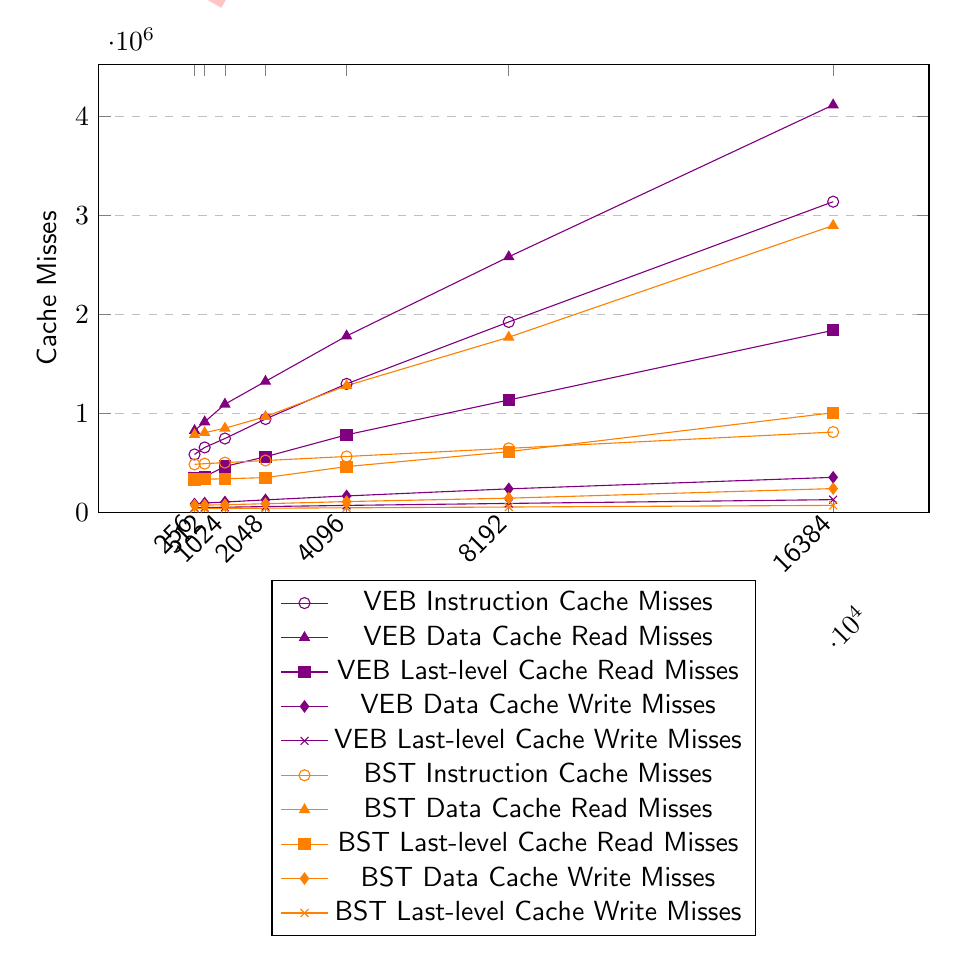
\begin{tikzpicture}
        \begin{axis}[
            width=\textwidth,
            height=0.6\textwidth,
            xlabel={Block Size},
            ylabel={Cache Misses},
            xtick={256, 512, 1024, 2048, 4096, 8192, 16384},
            xticklabels={256, 512, 1024, 2048, 4096, 8192, 16384},
            ymin=0,
            ymajorgrids=true,
            grid style=dashed,
            cycle list name=color list,
            enlarge x limits=0.15,
            xticklabel style={rotate=45, anchor=east},
            legend style={at={(0.5,-0.15)},anchor=north}
        ]
        \addplot+[mark=o, color=violet] table[x index=0, y index=1, col sep=comma] {
            BlockSize,InstructionCacheMisses
            256,586338
            512,656874
            1024,747164
            2048,944139
            4096,1298782
            8192,1923825
            16384,3138048
        };
        \addplot+[mark=triangle*, color=violet] table[x index=0, y index=1, col sep=comma] {
            BlockSize,DataCacheReadMisses
            256,826978
            512,914641
            1024,1093725
            2048,1323708
            4096,1782222
            8192,2581843
            16384,4114636
        };
        \addplot+[mark=square*, color=violet] table[x index=0, y index=1, col sep=comma] {
            BlockSize,LastLevelCacheReadMisses
            256,342641
            512,362002
            1024,465148
            2048,563046
            4096,784288
            8192,1136228
            16384,1839706
        };
        \addplot+[mark=diamond*, color=violet] table[x index=0, y index=1, col sep=comma] {
            BlockSize,DataCacheWriteMisses
            256,86317
            512,95840
            1024,105986
            2048,127986
            4096,167471
            8192,239100
            16384,355242
        };
        \addplot+[mark=x, color=violet] table[x index=0, y index=1, col sep=comma] {
            BlockSize,LastLevelCacheWriteMisses
            256,48242
            512,50590
            1024,53554
            2048,60146
            4096,71901
            8192,91876
            16384,130123
        };
        \addplot+[mark=o, color=orange] table[x index=0, y index=1, col sep=comma] {
            BlockSize,InstructionCacheMisses
            256,486541
            512,493182
            1024,503951
            2048,525072
            4096,565804
            8192,648061
            16384,812394
        };
        \addplot+[mark=triangle*, color=orange] table[x index=0, y index=1, col sep=comma] {
            BlockSize,DataCacheReadMisses
            256,786192
            512,806564
            1024,850909
            2048,967983
            4096,1280734
            8192,1769552
            16384,2897689
        };
        \addplot+[mark=square*, color=orange] table[x index=0, y index=1, col sep=comma] {
            BlockSize,LastLevelCacheReadMisses
            256,333316
            512,336076
            1024,340758
            2048,352443
            4096,463768
            8192,614714
            16384,1007555
        };
        \addplot+[mark=diamond*, color=orange] table[x index=0, y index=1, col sep=comma] {
            BlockSize,DataCacheWriteMisses
            256,72848
            512,74668
            1024,78745
            2048,88967
            4096,110487
            8192,145009
            16384,241735
        };
        \addplot+[mark=x, color=orange] table[x index=0, y index=1, col sep=comma] {
            BlockSize,LastLevelCacheWriteMisses
            256,40881
            512,41268
            1024,42107
            2048,43857
            4096,47511
            8192,55565
            16384,72183
        };
        \legend{VEB Instruction Cache Misses,
                VEB Data Cache Read Misses,
                VEB Last-level Cache Read Misses,
                VEB Data Cache Write Misses,
                VEB Last-level Cache Write Misses,
                BST Instruction Cache Misses,
                BST Data Cache Read Misses,
                BST Last-level Cache Read Misses,
                BST Data Cache Write Misses,
                BST Last-level Cache Write Misses}
        \end{axis}
    \end{tikzpicture}
    \caption{Cache misses for VEB and BST}
    \label{fig:cache_misses}
\end{figure}

\subsection{Time Analysis}
The following plot shows the time taken for insert and search operations for Van Emde-Boas trees and binary search trees. The full code for generating this plot is provided in the appendix \ref{appendix:time_performance_plot}.
\begin{figure}[h]
\centering
    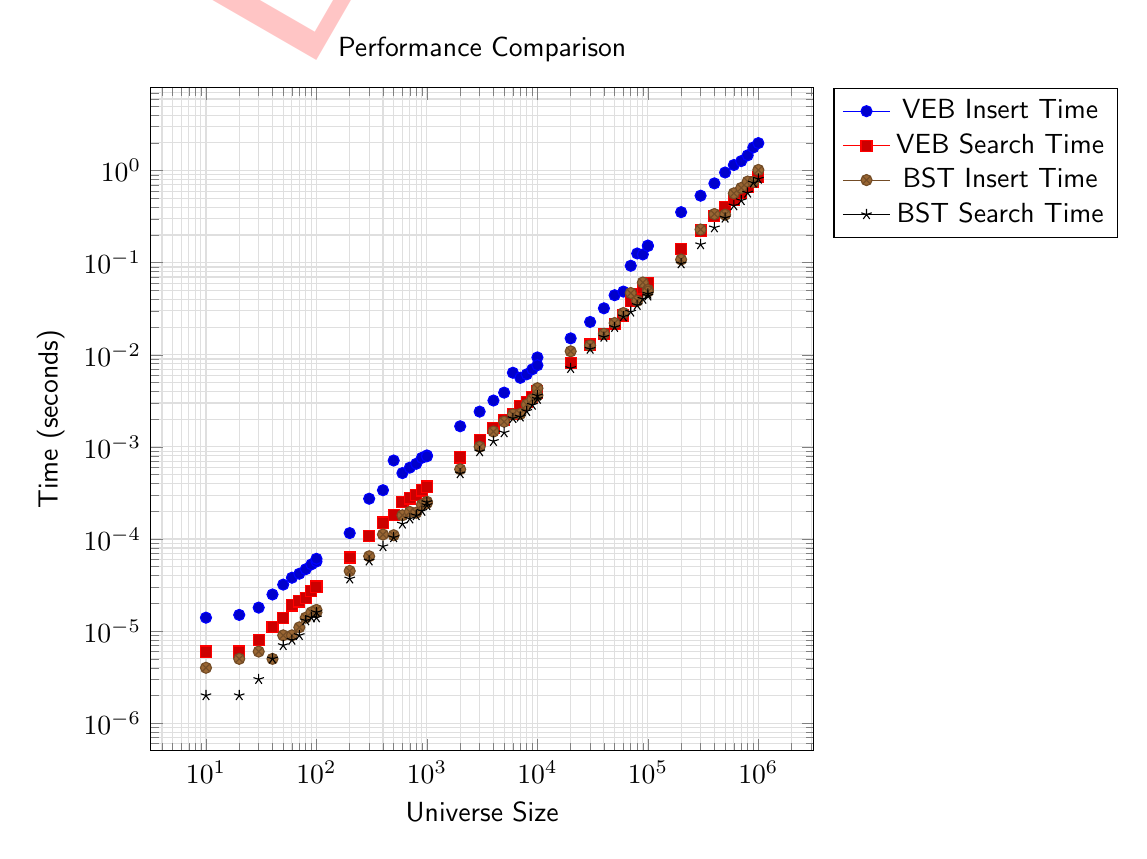
\begin{tikzpicture}
        \begin{axis}[
            title={Performance Comparison},
            xlabel={Universe Size},
            ylabel={Time (seconds)},
            xmode=log,
            ymode=log,
            legend pos=outer north east,
            grid=both,
            minor grid style={gray!25},
            major grid style={gray!25},
            width=10cm,
            height=10cm,
        ]

        \addplot coordinates {
        
            (10, 1.4000000000000123e-05)
        
            (20, 1.4999999999994185e-05)
        
            (30, 1.8000000000004124e-05)
        
            (40, 2.4999999999997247e-05)
        
            (50, 3.199999999999731e-05)
        
            (60, 3.800000000000331e-05)
        
            (70, 4.200000000000037e-05)
        
            (80, 4.700000000000537e-05)
        
            (90, 5.300000000000443e-05)
        
            (100, 5.7000000000001494e-05)
        
            (100, 6.0999999999998555e-05)
        
            (200, 0.00011600000000000499)
        
            (300, 0.00027399999999999647)
        
            (400, 0.000338999999999999)
        
            (500, 0.0007119999999999974)
        
            (600, 0.0005199999999999996)
        
            (700, 0.0005959999999999924)
        
            (800, 0.0006560000000000038)
        
            (900, 0.0007619999999999988)
        
            (1000, 0.0008089999999999903)
        
            (1000, 0.000791)
        
            (2000, 0.001676999999999998)
        
            (3000, 0.0024180000000000035)
        
            (4000, 0.0031909999999999994)
        
            (5000, 0.0038880000000000026)
        
            (6000, 0.006389000000000006)
        
            (7000, 0.005627999999999994)
        
            (8000, 0.006143999999999983)
        
            (9000, 0.006963999999999998)
        
            (10000, 0.009372999999999992)
        
            (10000, 0.00770800000000002)
        
            (20000, 0.015093999999999996)
        
            (30000, 0.02276600000000001)
        
            (40000, 0.032016000000000044)
        
            (50000, 0.04438800000000004)
        
            (60000, 0.04861599999999999)
        
            (70000, 0.09270800000000001)
        
            (80000, 0.12599899999999997)
        
            (90000, 0.12299899999999986)
        
            (100000, 0.15362199999999993)
        
            (100000, 0.15198299999999998)
        
            (200000, 0.3541810000000001)
        
            (300000, 0.5345530000000003)
        
            (400000, 0.7273519999999998)
        
            (500000, 0.9544100000000002)
        
            (600000, 1.151159999999999)
        
            (700000, 1.2694739999999989)
        
            (800000, 1.466095000000001)
        
            (900000, 1.784718999999999)
        
            (1000000, 1.9902820000000006)
        
        };
        \addlegendentry{VEB Insert Time}

        \addplot coordinates {
        
            (10, 5.999999999999062e-06)
        
            (20, 6.0000000000060005e-06)
        
            (30, 7.999999999994123e-06)
        
            (40, 1.1000000000004062e-05)
        
            (50, 1.4000000000000123e-05)
        
            (60, 1.8999999999998185e-05)
        
            (70, 2.1000000000000185e-05)
        
            (80, 2.2999999999995246e-05)
        
            (90, 2.6999999999999247e-05)
        
            (100, 3.099999999999631e-05)
        
            (100, 3.0000000000002247e-05)
        
            (200, 6.300000000000056e-05)
        
            (300, 0.00010800000000000393)
        
            (400, 0.00015099999999999836)
        
            (500, 0.00018399999999999667)
        
            (600, 0.0002530000000000032)
        
            (700, 0.00027599999999999847)
        
            (800, 0.0003010000000000096)
        
            (900, 0.0003369999999999901)
        
            (1000, 0.00038000000000000533)
        
            (1000, 0.0003700000000000092)
        
            (2000, 0.0007690000000000058)
        
            (3000, 0.0011820000000000025)
        
            (4000, 0.0016019999999999923)
        
            (5000, 0.0019639999999999935)
        
            (6000, 0.0022979999999999945)
        
            (7000, 0.0027810000000000057)
        
            (8000, 0.0030930000000000124)
        
            (9000, 0.003485999999999989)
        
            (10000, 0.0038930000000000076)
        
            (10000, 0.0040869999999999795)
        
            (20000, 0.008152999999999994)
        
            (30000, 0.012925999999999993)
        
            (40000, 0.016742999999999952)
        
            (50000, 0.02147199999999999)
        
            (60000, 0.026714999999999933)
        
            (70000, 0.038515999999999995)
        
            (80000, 0.0455890000000001)
        
            (90000, 0.05261999999999989)
        
            (100000, 0.06001699999999999)
        
            (100000, 0.06068499999999988)
        
            (200000, 0.14119400000000004)
        
            (300000, 0.22347599999999979)
        
            (400000, 0.3185880000000001)
        
            (500000, 0.4023570000000003)
        
            (600000, 0.48375900000000094)
        
            (700000, 0.5740680000000005)
        
            (800000, 0.6603290000000008)
        
            (900000, 0.7571050000000028)
        
            (1000000, 0.8561949999999996)
        
        };
        \addlegendentry{VEB Search Time}

        \addplot coordinates {
        
            (10, 3.9999999999970615e-06)
        
            (20, 4.9999999999980616e-06)
        
            (30, 5.999999999999062e-06)
        
            (40, 5.0000000000050004e-06)
        
            (50, 8.999999999995123e-06)
        
            (60, 8.999999999995123e-06)
        
            (70, 1.1000000000004062e-05)
        
            (80, 1.4000000000000123e-05)
        
            (90, 1.5999999999995185e-05)
        
            (100, 1.6000000000002124e-05)
        
            (100, 1.7000000000003124e-05)
        
            (200, 4.499999999999643e-05)
        
            (300, 6.499999999999562e-05)
        
            (400, 0.00011200000000000099)
        
            (500, 0.00010999999999999899)
        
            (600, 0.0001810000000000006)
        
            (700, 0.00019700000000000273)
        
            (800, 0.00019299999999999873)
        
            (900, 0.0002349999999999991)
        
            (1000, 0.00025399999999999034)
        
            (1000, 0.0002459999999999962)
        
            (2000, 0.0005719999999999892)
        
            (3000, 0.001003999999999991)
        
            (4000, 0.001467999999999997)
        
            (5000, 0.0018800000000000067)
        
            (6000, 0.002253999999999992)
        
            (7000, 0.0022830000000000072)
        
            (8000, 0.0028819999999999957)
        
            (9000, 0.0032899999999999874)
        
            (10000, 0.0036299999999999943)
        
            (10000, 0.0043400000000000105)
        
            (20000, 0.010914000000000007)
        
            (30000, 0.012635000000000007)
        
            (40000, 0.016928)
        
            (50000, 0.02214900000000003)
        
            (60000, 0.028437000000000046)
        
            (70000, 0.04689299999999996)
        
            (80000, 0.03850500000000001)
        
            (90000, 0.06102699999999994)
        
            (100000, 0.050748000000000015)
        
            (100000, 0.04854199999999986)
        
            (200000, 0.10826499999999983)
        
            (300000, 0.22938499999999973)
        
            (400000, 0.3380030000000005)
        
            (500000, 0.33224699999999974)
        
            (600000, 0.5672859999999993)
        
            (700000, 0.649248)
        
            (800000, 0.7613050000000001)
        
            (900000, 0.7526459999999986)
        
            (1000000, 1.0174859999999981)
        
        };
        \addlegendentry{BST Insert Time}

        \addplot coordinates {
        
            (10, 2.000000000002e-06)
        
            (20, 1.9999999999950613e-06)
        
            (30, 3.0000000000030003e-06)
        
            (40, 4.9999999999980616e-06)
        
            (50, 7.000000000000062e-06)
        
            (60, 8.000000000001062e-06)
        
            (70, 8.999999999995123e-06)
        
            (80, 1.2999999999999123e-05)
        
            (90, 1.4000000000000123e-05)
        
            (100, 1.4000000000000123e-05)
        
            (100, 1.6000000000002124e-05)
        
            (200, 3.700000000000231e-05)
        
            (300, 5.8000000000002494e-05)
        
            (400, 8.299999999999974e-05)
        
            (500, 0.00010399999999999993)
        
            (600, 0.0001460000000000003)
        
            (700, 0.00016599999999999948)
        
            (800, 0.0001799999999999996)
        
            (900, 0.00020100000000000673)
        
            (1000, 0.00023200000000000998)
        
            (1000, 0.0002500000000000002)
        
            (2000, 0.0005140000000000006)
        
            (3000, 0.0008900000000000019)
        
            (4000, 0.0011530000000000012)
        
            (5000, 0.0014300000000000007)
        
            (6000, 0.002041000000000001)
        
            (7000, 0.002117999999999981)
        
            (8000, 0.0024379999999999957)
        
            (9000, 0.0028499999999999914)
        
            (10000, 0.0033030000000000004)
        
            (10000, 0.003594999999999987)
        
            (20000, 0.007138999999999979)
        
            (30000, 0.01154299999999997)
        
            (40000, 0.015600000000000003)
        
            (50000, 0.019917000000000018)
        
            (60000, 0.025976)
        
            (70000, 0.02924899999999997)
        
            (80000, 0.03455000000000008)
        
            (90000, 0.040310999999999986)
        
            (100000, 0.04578100000000007)
        
            (100000, 0.043630999999999975)
        
            (200000, 0.09770000000000012)
        
            (300000, 0.157721)
        
            (400000, 0.24025300000000005)
        
            (500000, 0.3063980000000006)
        
            (600000, 0.41637599999999964)
        
            (700000, 0.4742290000000011)
        
            (800000, 0.5724750000000007)
        
            (900000, 0.7364999999999995)
        
            (1000000, 0.8112259999999978)
        
        };
        \addlegendentry{BST Search Time}

        \end{axis}
    \end{tikzpicture}
\caption{Time analysis}
\end{figure}

\newpage
\section{Observations}

Based on the experimental results, we observe the following:

\begin{itemize}
\item \textbf{Cache Misses Increase}: Contrary to expectations, the Van Emde-Boas tree consistently shows more cache misses compared to the binary search tree across all tested universe sizes.
\item \textbf{Scalability Issue}: As the universe size increases, the difference in cache performance becomes more pronounced, but not in the expected way. The vEB trees exhibit worse scalability in terms of cache efficiency compared to BSTs.
\item \textbf{Complexity without Benefit}: While vEB trees are indeed more complex to implement and manage, this complexity does not translate into better performance. In fact, BSTs outperform vEB trees in terms of cache efficiency, making them a preferable choice despite their simpler structure.
\end{itemize}

These findings contradict the hypothesis that Van Emde-Boas trees are more efficient in terms of cache usage. Instead, they indicate that binary search trees may offer better performance in practical scenarios due to their simpler and more effective memory access patterns.\\

The ethics of scientific research demand unwavering rigor and integrity in conducting experiments and presenting results. It is crucial to respect the outcomes obtained, even if they do not confirm initial hypotheses or seem unconvincing. Attempting to redo the experiment solely to alter or manipulate the results to fit preconceived expectations is a severe violation of ethical principles.\\

In analyzing the results of our experiments, several potential causes of error must be considered to understand why the expected outcomes were not achieved. Firstly, the implementation of the Van Emde-Boas (vEB) tree might have contained inefficiencies or bugs that increased the number of cache misses. This could stem from incorrect handling of memory allocations or suboptimal recursive function calls. Secondly, the experimental setup and measurement process might have introduced biases. For instance, variations in the hardware environment, even when controlled through Docker, could affect cache performance. Thirdly, the sample sizes and the specific input data used in the tests might not have been representative, leading to skewed results. Lastly, theoretical advantages of vEB trees might not translate into practical performance gains due to overheads not accounted for in theoretical models, such as those related to memory access patterns and cache line utilization. These factors collectively contribute to the discrepancy between the hypothesized and observed outcomes.

\section{Appendix}
\subsection{Ven Emde-Boas Trees implementation}
\label{appendix:veb}
\lstinputlisting[language=Python, caption=Van Emde-Boas Trees]{../van_emde_boas_tree.py}

\subsection{Binary Search Trees implementation}
\label{appendix:bst}
\lstinputlisting[language=Python, caption=Binary Search Trees]{../binary_search_tree.py}

\subsection{Time performance plot}
\label{appendix:time_performance_plot}
\lstinputlisting[language=Python, caption=Time performance plot]{../performances.py}
\newpage
\listoffigures
\lstlistoflistings
\end{document}
